\section{QGIS}
QGIS adalah perangkat Sistem Informasi Geografis (SIG) Open Source yang user friendly dengan lisensi di bawah GNU General Public License. QGIS merupakan proyek tidak resmi dari Open Source Geospatial Foundation (OSGeo). QGIS dapat dijalankan pada Linux, Unix, Mac OSX, Windows dan Android, serta mendukung banyak format dan fungsionalitas data vektor, raster, dan basisdata.
Quantum GIS mendukung penggunaan "GPS tools" untuk menggunggah (upload) atau mengunduh (download) data langsung ke unit GPS. Pengguna juga dapat mengkonversi format-format GPS ke format GPX atau melakukan import dan export terhadap data format GPX yang ada.
Andaikan pengguna memiliki sebuah web server yang telah terpasang fitur UMN MapServer, pengguna dapat menpublikasi map di internet untuk berbagi (sharing) dengan pengguna lainnya.

\subsection{Getting QGIS}
\begin{enumerate}
\item
Buka browser internet Anda dan ketikkan pada bagian atas jendela browser Anda dengan tulisan qgis.org. Kemudian tekan Enter.\ref{image1}.
\begin{figure}[ht]
        \centerline{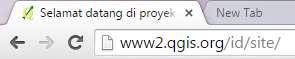
\includegraphics[width=0.25\textwidth]{figures/image1}}
        \caption{gambar}
        \label{image1}
        \end{figure}

Situs resmi QGIS akan terlihat seperti ini:\ref{image2}.
\begin{figure}[ht]
        \centerline{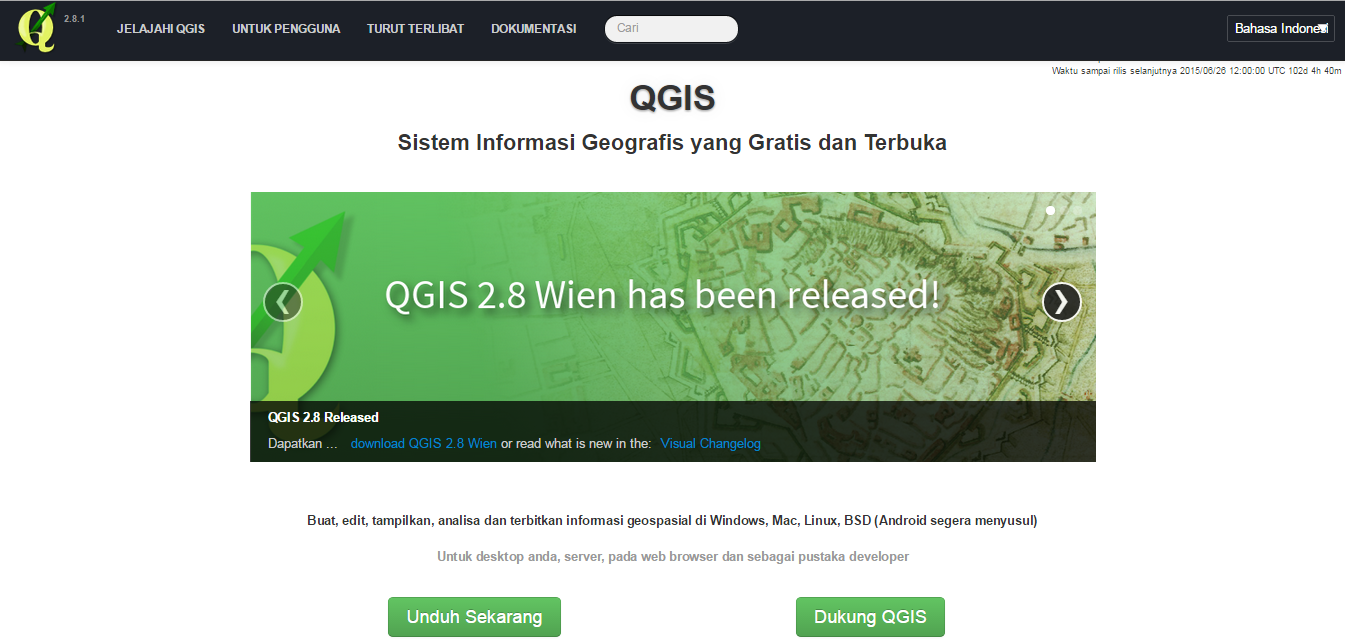
\includegraphics[width=1.00\textwidth]{figures/image2}}
        \caption{gambar}
        \label{image2}
        \end{figure}
\item
Klik Unduh Sekarang
\item
Jika Anda menggunakan Windows, klik pada QGIS Standalone Installer Version 2.8 (32 bit). Nomor versi komputer Anda mungkin berbeda.\ref{image3}.
\begin{figure}[ht]
        \centerline{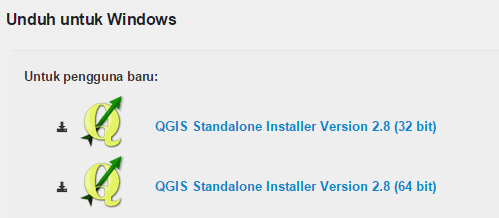
\includegraphics[width=0.25\textwidth]{figures/image3}}
        \caption{gambar}
        \label{image3}
        \end{figure}
\item
Jika Anda tidak menggunakan Windows, pilih Sistem Operasi Anda dari menu yang tersedia. Ikuti intruksi instalasi.\ref{image4}.
\begin{figure}[ht]
        \centerline{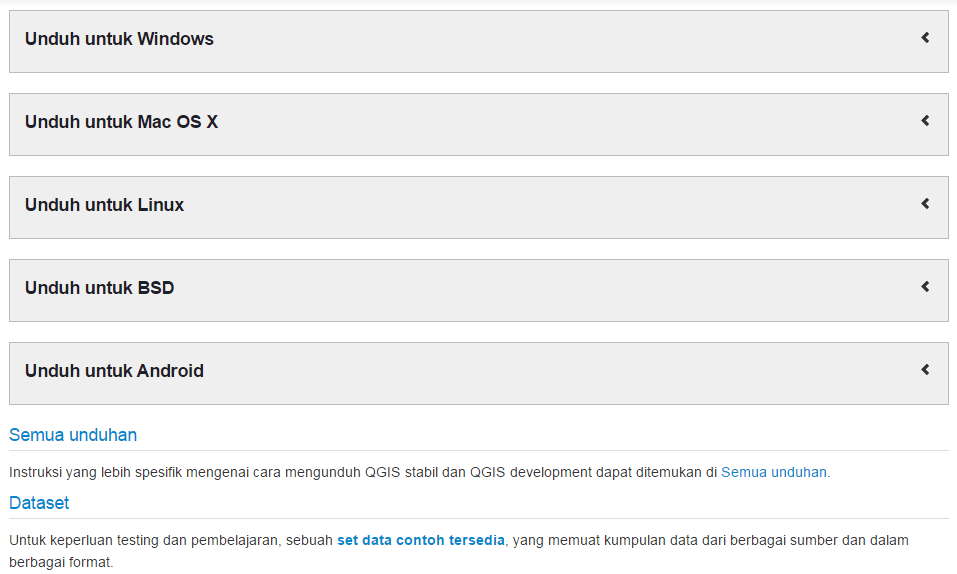
\includegraphics[width=0.25\textwidth]{figures/image4}}
        \caption{gambar}
        \label{image4}
        \end{figure}
\item
Ketika file selesai didownload, jalankan dan ikuti perintah untuk menginstal QGIS.
\end{enumerate}

\subsection{Installing QGIS}
\begin{enumerate}
\item
Buka folder dimana anda menyimpan file instalasi QGIS.\ref{image5}.
\begin{figure}[ht]
        \centerline{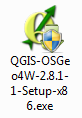
\includegraphics[width=0.05\textwidth]{figures/image5}}
        \caption{gambar}
        \label{image5}
        \end{figure}
\item
Jalankan file instalasi tersebut. Jika Anda menginstal QGIS versi 2.x, akan terlihat seperti ini:\ref{image6}.
\begin{figure}[ht]
        \centerline{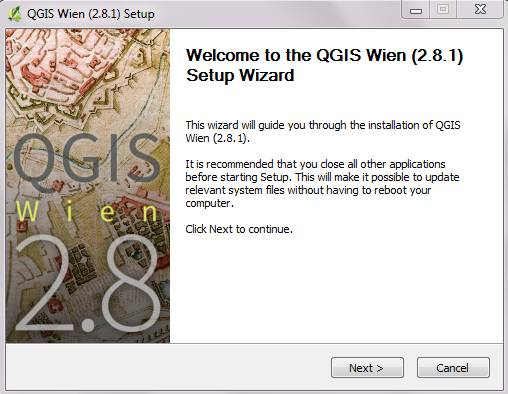
\includegraphics[width=0.25\textwidth]{figures/image6}}
        \caption{gambar}
        \label{image6}
        \end{figure}
\item 
Klik Next
\item
Klik I Agree untuk setuju dengan syarat dan ketentuan yang berlaku.\ref{image7}.
\begin{figure}[ht]
        \centerline{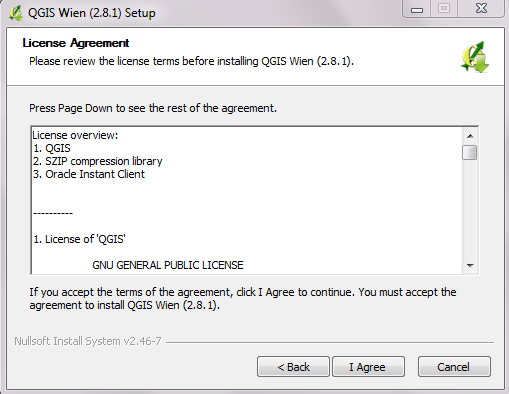
\includegraphics[width=0.25\textwidth]{figures/image7}}
        \caption{gambar}
        \label{image7}
        \end{figure}
\item
Pada jendela berikutnya Anda akan ditanyakan dimana Anda akan menginstall QGIS. Pada kasus umum, pengaturan bawaan yang ada sudah dapat digunakan. Klik Next.\ref{image8}.
\begin{figure}[ht]
        \centerline{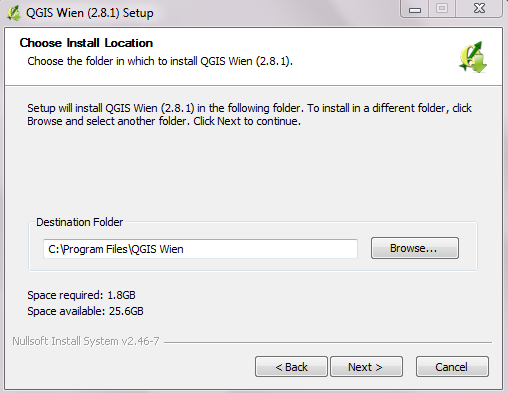
\includegraphics[width=0.25\textwidth]{figures/image8}}
        \caption{gambar}
        \label{image8}
        \end{figure}
\item
Pada jendela berikutnya, klik Install tanpa mencentang apapun yang ada di dalam kotak.\ref{image9}.
\begin{figure}[ht]
        \centerline{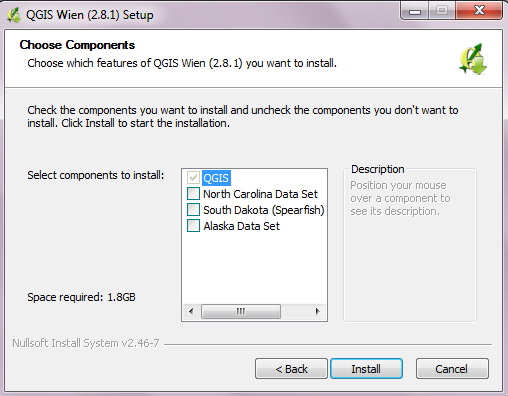
\includegraphics[width=0.25\textwidth]{figures/image9}}
        \caption{gambar}
        \label{image9}
        \end{figure}

QGIS akan memulai untuk menginstall. Ini mungkin akan membutuhkan beberapa waktu untuk selesai.\ref{image10}.
\begin{figure}[ht]
        \centerline{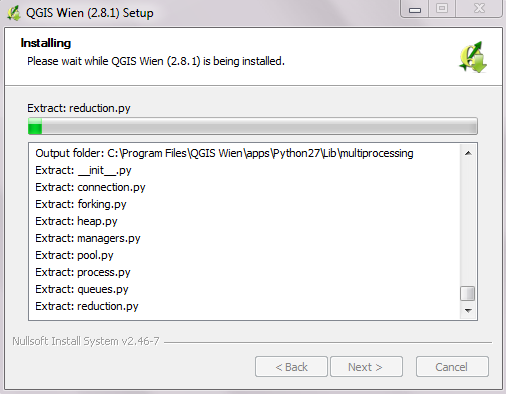
\includegraphics[width=0.25\textwidth]{figures/image10}}
        \caption{gambar}
        \label{image10}
        \end{figure}
\item
Klik Finish untuk melengkapi instalasi. Kemudian komputer Anda akan me-reboot secara otomatis.\ref{image11}.
\begin{figure}[ht]
        \centerline{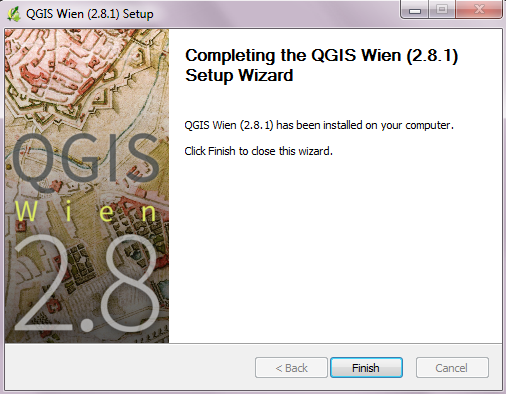
\includegraphics[width=0.25\textwidth]{figures/image11}}
        \caption{gambar}
        \label{image11}
        \end{figure}
\item
Buka QGIS dari Start Menu, berikut tampilan QGIS.\ref{image12}.
\begin{figure}[ht]
        \centerline{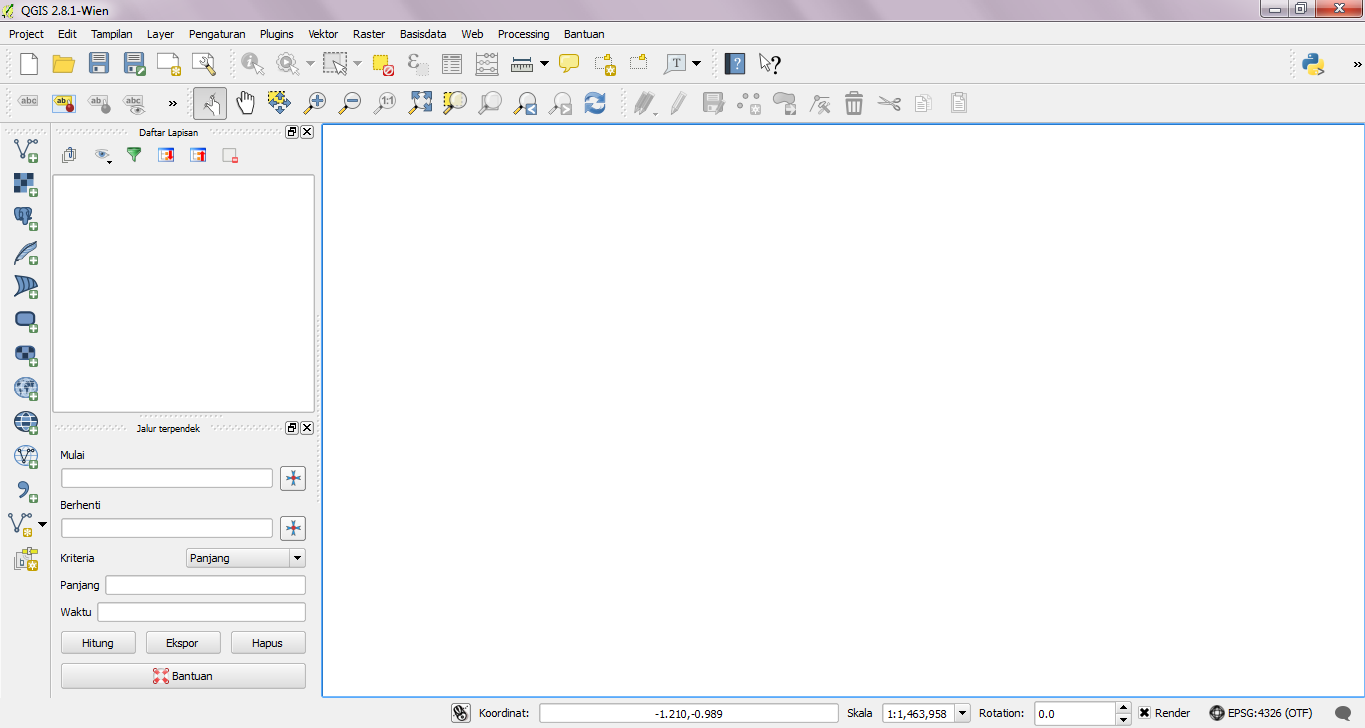
\includegraphics[width=0.25\textwidth]{figures/image12}}
        \caption{gambar}
        \label{image12}
        \end{figure}
\end{enumerate}


\subsection{Toolbar}
Pada bagian atas dari tampilan QGIS terdapat banyak sekali tool, dimana masing-masing tool tersebut masuk ke dalam beberapa kategori “toolbar”. Sebagai contoh,  file mengizinkan Anda untuk menyimpan, membuka, mencetak dan memulai proyek baru. Kita telah menggunakan salah satu alat dari toolbar file ketika kita membuka proyek baru.\ref{toolbar}.
\begin{figure}[ht]
    \centerline{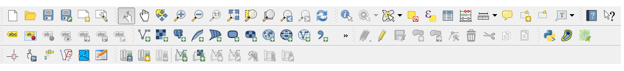
\includegraphics[width=0.25\textwidth]{figures/toolbar.png}}
    \caption{gambar toolbar yang ada pada QGis}
    \label{toolbar}
    \end{figure}

Dengan menggerakkan mouse ke atas ikon, nama tool akan muncul untuk membantu mengidentifikasi setiap tool. Jumlah tool yang ada (tombol) akan tampak sangat banyak pada awalnya, tapi Anda perlahan akan mengenalnya. Tool yang ada dikelompokkan sesuai dengan fungsi pada toolbars. Jika Anda melihat lebih dekat, Anda akan melihat titik-titik vertikal sejumlah sepuluh titik pada bagian kiri dari setiap toolbar. Jika Anda meng-klik dan menahannya dengan menggunakan mouse ,dapat menggerakkan toolbar ke tempat yang lebih sesuai atau memisahkannnya sesuai.\ref{toolbar1}.
\begin{figure}[ht]
    \centerline{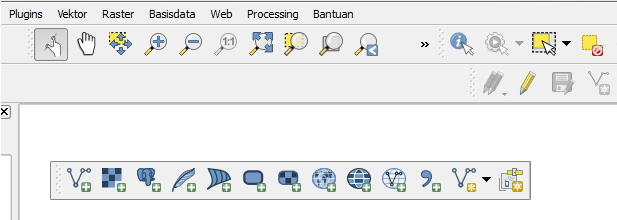
\includegraphics[width=0.25\textwidth]{figures/toolbar1.png}}
    \caption{gambar toolbar yang ada pada QGis}
    \label{toolbar1}
    \end{figure}

\section{Label Tool}
Label dapat ditambahkan ke dalam peta untuk menunjukkan informasi tentang objek. Suatu layer vektor dapat memiliki label yang berkaitan dengan layer tersebut. Label bergantung pada data atribut dari layer terkait.
Ada beberapa cara untuk menambahkan label pada QGIS, tetapi beberapa cara lebih baik dibandingkan yang lain. Dapat dilihat ketika membuka jendela properti dari sebuah layer, terdapat tabs yang bertuliskan "Labels". Walaupun tab ini dirancang untuk memberikan label pada peta yang dibuat, tab ini fungsinya tidak sebaik "Tool Label", yang akan dipelajari pada bagian ini. Sebelum mengakses Tool Label, harus dipastikan bahwa fitur tersebut telah diaktifkan. Berikut langkah-langkahnya :
\begin{enumerate}
\item
Pergi ke menu item View --> Toolbars
\item
Pastikan item Label telah memiliki tanda centang disebelahnya. Jika belum, klik pada item Label dan fitur tersebut akan diaktifkan.\ref{label}.
\begin{figure}[ht]
    \centerline{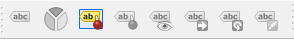
\includegraphics[width=0.25\textwidth]{figures/label.png}}
    \caption{Toolbar Label tampak seperti ini}
    \label{label}
    \end{figure}
\item
Klik layer POI\_Bandung\_OSM yang terdapat pada panel Daftar Layer, sehingga layer tersebut tersorot
\end{enumerate}
